\chapter{Manuel Utilisateur}

\section{Application Android}

L'application Android permet à l'utilisateur de suivre son trajet sur une carte Google Maps et de faire une course contre un autre trajet.

Tout d'abord, lors du lancement de l'application, il faut se connecter avec son identifiant et son mot de passe pour arriver sur la carte. La navigation se fait avec trois onglets. Le premier onglet correspond à la carte où l'on peut voir sa position et de plus le trajet que l'on est en train de faire durant une course.

Le deuxième onglet montre toutes les catégories que l'utilisateur a créé et il peut en créer de nouvelles. Dans ces catégories, l'utilisateur peut choisir le trajet contre lequel il veut faire la course.

Et enfin le troisième onglet correspond à la page des options où l'utilisateur peut par exemple changer le thème de la carte en plus sombre (une actualisation de la position sur la carte est nécessaire pour que le thème change) ou encore se déconnecter.

\section{Site web}

Le site web a une interface très simple d'utilisation. La page d'accueil décrit très simplement le but de l'application GhostRun.

En haut à gauche de la page d'accueil, nous avons deux boutons, Espace membres et préférences, qui ne sont disponibles que si l'utilisateur s'est connecté. Il peut le faire avec le bouton Connexion en haut à droite. Les identifiants de l'utilisateur sont les mêmes que ceux sur l'application. Si un utilisateur essaye d'accéder à l'une de ces pages sans être connecté, il sera redirigé sur la page de connexion.

Après s'être connecté, l'utilisateur a donc accès à son espace membres où il peut voir tous les trajets qu'il a réalisé dans chacune de ses catégories. En cliquant sur l'un des trajets, il peut voir plusieurs statistiques sur ce trajet (comme la distance parcourue, sa vitesse moyenne, la durée du trajet, ou encore un graphique du dénivelé). Il peut aussi bien évidemment consulter l'itinéraire parcouru sur la carte à gauche de la page. Tout ceci peut lui permettre de faire son choix sur quel trajet il souhaite réaliser une course.

Et enfin, la page des préférences où l'utilisateur peut contrôler un ensemble de réglages concernant son compte, qui restent pour l'instant à déterminer. 

\section{Interface administrateur}

L'interface administrateur permet aux administrateur de consulter la base de données depuis une interface plus agréable que des commandes SQL. Elle est générée dynamiquement en fonction des tables définies. Elle permet d'ajouter, de supprimer ou de modifier les données concernant n'importe quel trajet ou catégorie de n'importe quel utilisateur. Son accès est réservé aux comptes disposant de l'attribut "super-utilisateur".

\begin{figure}[h]
    \centering
    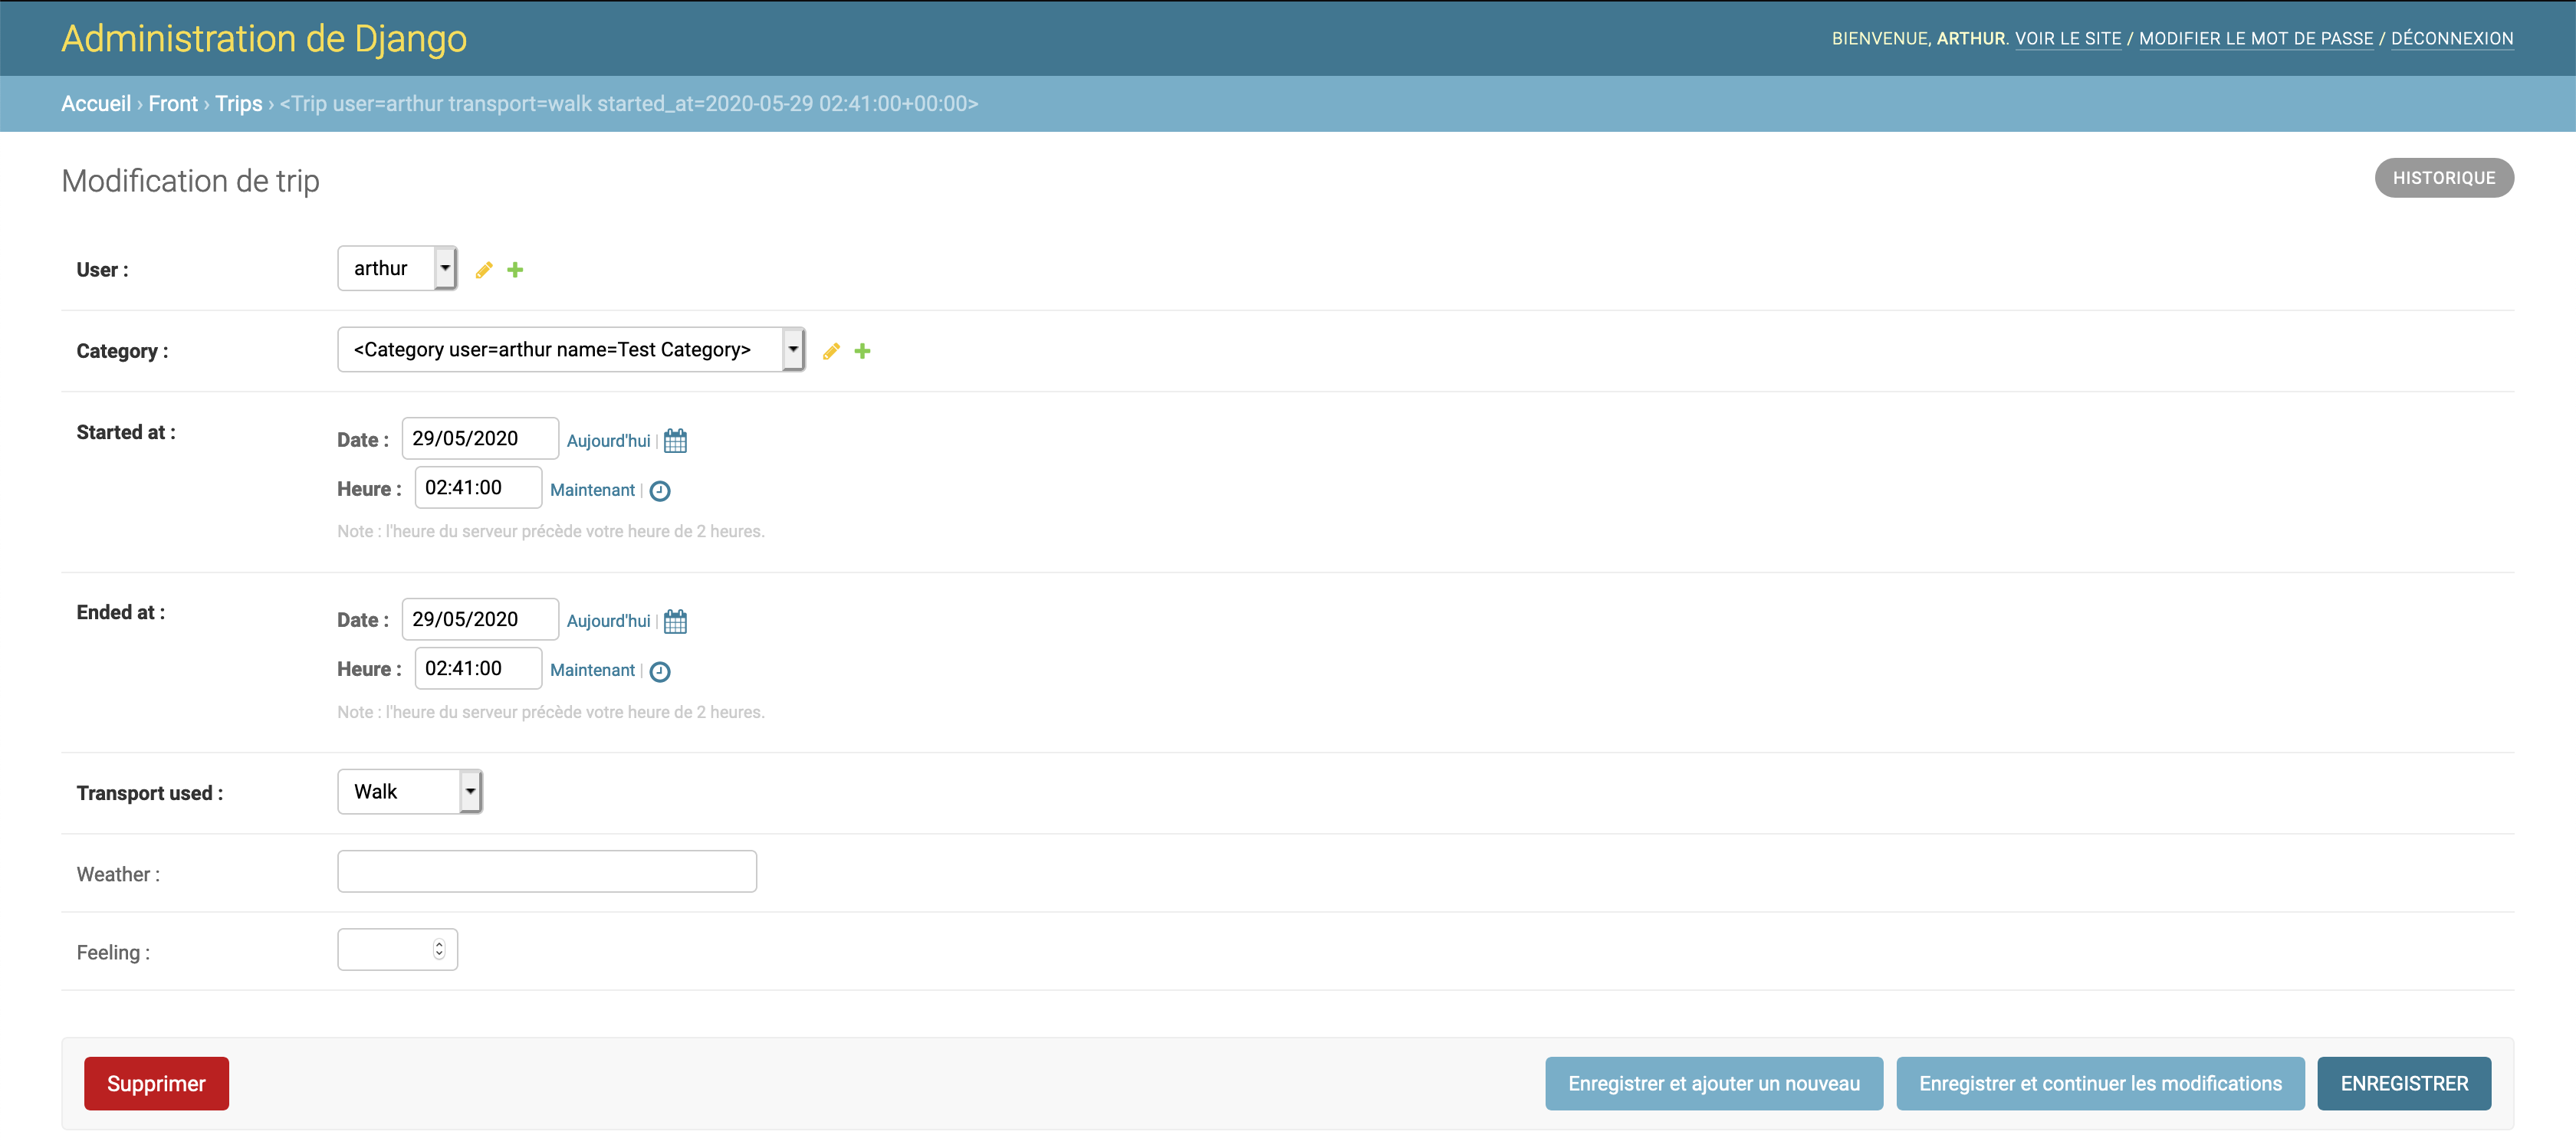
\includegraphics[keepaspectratio, width=2\textwidth/2, height=2\textheight/5]{ima/interface-admin}
    \caption{L'interface administrateur en images.}
    \label{fig:80-interface-administrateur}
\end{figure}


\section{API}

L'API est une interface permettant à des services externes de se connecter au site web et de lui communiquer des données, ou d'en récupérer. Un utilisateur souhaitant utiliser l'API, par exemple à travers l'application téléphone, devra se connecter avec son utilisateur et son mot de passe.
L'API suit les normes REST usuelles auxquelles on pourrait s'attendre d'un tel service. Par exemple, l'endpoint /trips contient la liste des trips et supporte GET, HEAD, et POST pour respectivement récupérer la liste des trajets de l'utilisateur connecté, en connaitre la date de dernière modification et en ajouter un.
Un trajet particulier, identifié par sa clé primaire dans l'URL, pourra être modifié (PATCH), remplacé (PUT), récupéré (GET) ou encore supprimé (DELETE).

Enfin, chaque route supporte la requête de type OPTIONS, qui permet de connaitre les éléments à passer à la route donnée, et les contraintes qui seront calculées.
Les codes de réponse HTTP sont utilisés par le serveur, qui pourra par exemple répondre 200 (OK) dans le cas ou la requête c'est bien passée, 201 (Created) si l'objet à été créé, 403 (Unauthorised) si l'utilisateur connecté ne peut accéder aux informations demandées, 400 (Bad Request) si les paramètres passés sont invalides, 429 (Rate-Limit Exceeded) si l'application à effectué trop de requêtes pendant une période, 404 (Not found) si la ressource demandée n'a pas été trouvée.

Enfin, l'API dispose d'une interface HTML permettant d'interagir facilement sans utiliser de logiciels spécialisés tels que Postman ou Curl. Son interface est visible dans la \autoref{fig:80-interface-API}.

\begin{figure}[h]
    \centering
    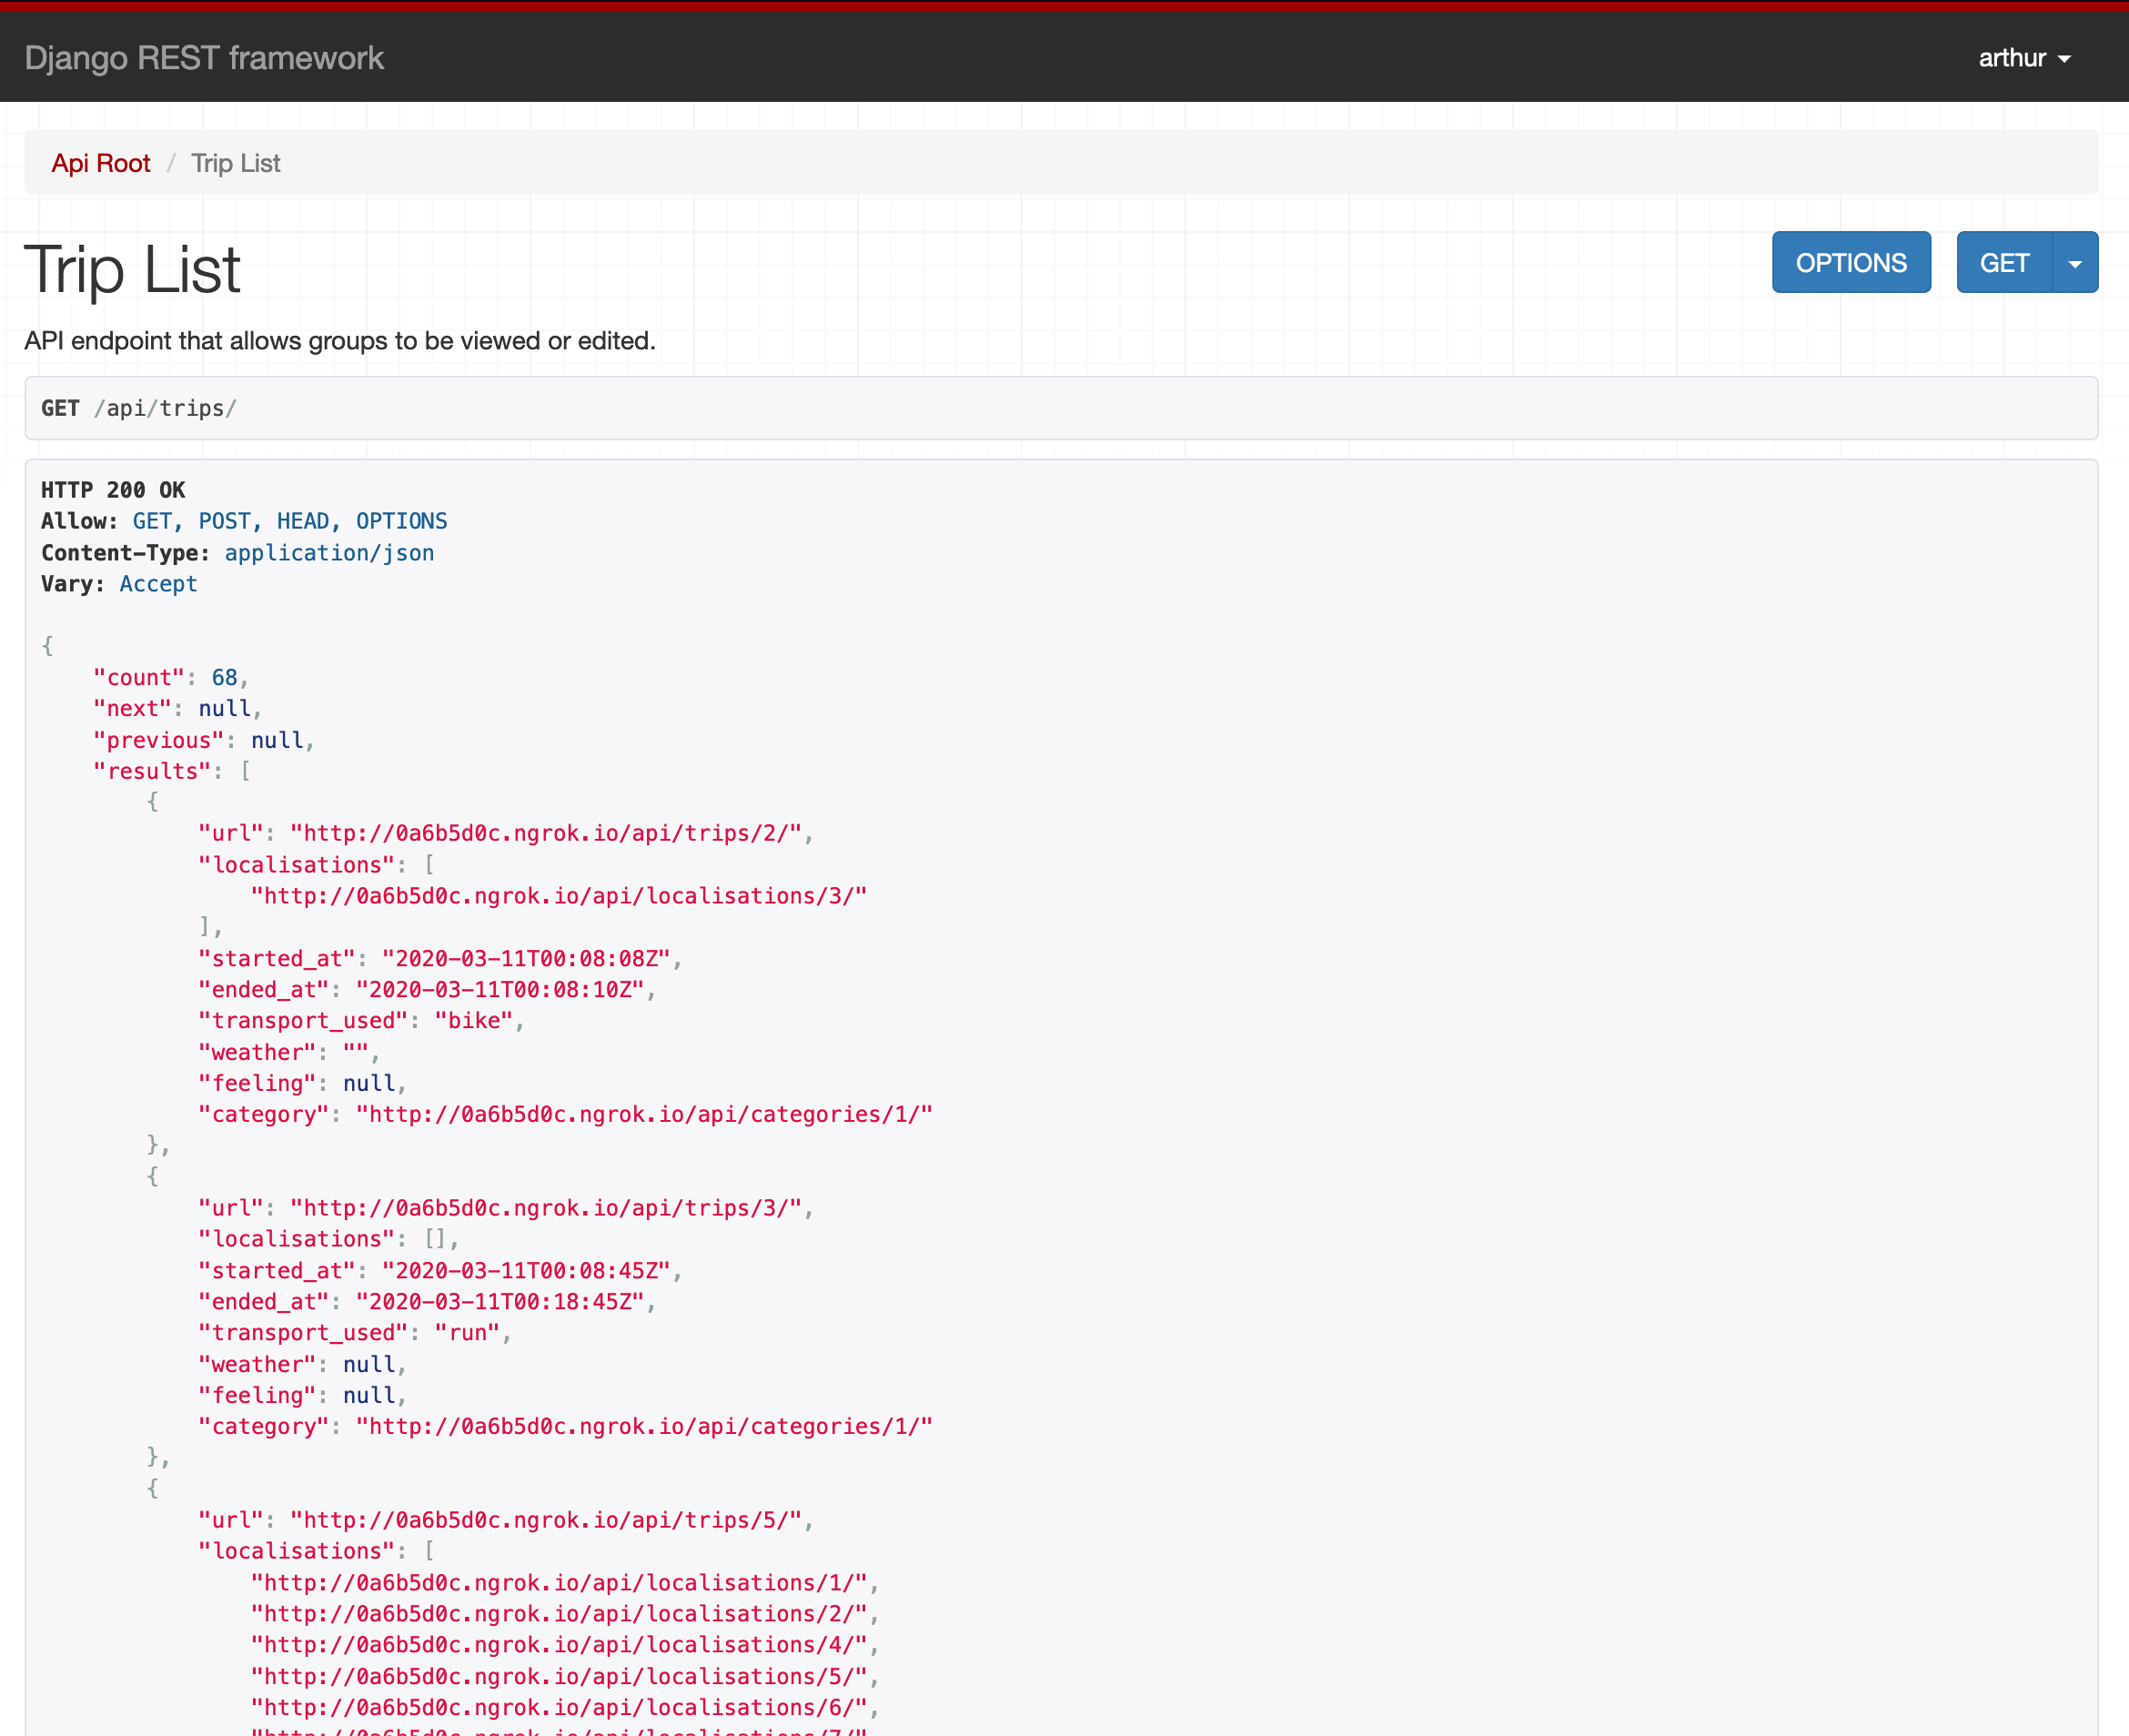
\includegraphics[keepaspectratio, width=2\textwidth/2, height=2\textheight/5]{ima/interface-api}
    \caption{L'interface de l'API utilisable pour le developpement.}
    \label{fig:80-interface-API}
\end{figure}
